
\documentclass[tikz, border=1mm]{standalone}

\usepackage{amsmath}

\usetikzlibrary{calc,angles,quotes}

\begin{document}
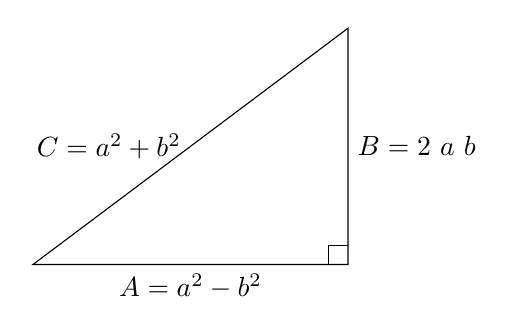
\begin{tikzpicture}[scale=1.0]

	\coordinate (A) at (0,0);
	\coordinate (B) at (4,0);
	\coordinate (C) at (4,3);

	% remaining side of triangle
	\draw (A) -- (B) -- (C) -- cycle;

	% sides
	\node[below] at ($(A)!0.5!(B)$) {$A = a^2 - b^2$};
	\node[right] at ($(B)!0.5!(C)$) {$B = 2 \ a \ b$};
	\node[left] at ($(A)!0.5!(C)$) {$C = a^2 + b^2$};

	% right angle
	\pic [draw, angle radius=7pt, angle eccentricity=1]
	{right angle = C--B--A};

\end{tikzpicture}
\end{document}
